%-------------------------------------------------------------------------------
% File: main.tex
%       Compile using:
%           $ pdflatex main.tex
%           $ biber main
%
% Author: Marco Pinna
%         Created on 14/07/2022
%-------------------------------------------------------------------------------
\documentclass[11pt, a4paper, twoside, openany]{book}

% equal left and right margins
\usepackage[hmarginratio=1:1]{geometry}

% configuration to typeset documents in english
\usepackage[english]{babel}
\usepackage{import}
% include graphics in the file
\usepackage{graphicx}
\usepackage{pgf}
\usepackage{tikz}
% used in the dedication environment definition
\usepackage{afterpage}

% used to set page background image
\usepackage{tikz}

% used to handle math equations and formulas
\usepackage{amsmath}
\usepackage{mathtools}
\usepackage{array}

% used to handle quotes
\usepackage{csquotes}

%used to handle bibliography
\usepackage[backend=bibtex,
style=alphabetic,
citestyle=authoryear
]{biblatex}
\addbibresource{references.bib}

%used to change color and background color of single words
\usepackage{xcolor}

%used to place figures side by side
\usepackage{subfig}

%used to fix figure positioning
\usepackage{float}

%used to reference sections
\usepackage{hyperref}

\usepackage{wrapfig}

\usepackage{blkarray}

\usepackage{hyperref}

\usepackage{dirtree}

% blank page command
\newcommand{\blankpage}
{
    \null
    \thispagestyle{empty}%
    \addtocounter{page}{-1}%
    \newpage
}
\newcommand\inputpgf[2]{{
\let\pgfimageWithoutPath\pgfimage
\renewcommand{\pgfimage}[2][]{\pgfimageWithoutPath[##1]{#1/##2}}
\input{#1/#2}
}}
% dedication environment
\newenvironment{dedication}
{
    % blank page before dedication
    \afterpage{\blankpage}
    % we want a new page
    \clearpage
    % no header and footer
    \thispagestyle{empty}
    % some space at the top
    \vspace*{\stretch{1}}
    % the text is in italics
    \itshape
    % flush to the right margin
    \raggedleft
    % blank page after dedication
    \afterpage{\blankpage}
}
{
    % end the paragraph
    \par
    % space at bottom is one times that at the top
    \vspace{\stretch{1}}
    % finish off the page
    \clearpage
}

\newenvironment{specifications}
{
	\fontfamily{qtm}\selectfont
}{\par}


%-------------------------------------------------------------------------------
% Title page
%-------------------------------------------------------------------------------
\title{
    \vspace{-3cm}
    
\includegraphics[scale=0.3]{img/cherubino_black.eps}\\
    {\scshape University of Pisa}\\
    School of Engineering\\
    \rule{7cm}{0.01cm}\\
    {\normalsize{\scshape Distributed Systems and Middleware Technologies}}\\
    [2cm]
    {\scshape DVoting - A distributed electronic voting system}\\
    [3cm]
    \LARGE{\textbf{Supervisors}\hfill\textbf{Students}}\\
    \Large{\emph{Alessio Bechini}\hfill\emph{Yuri Mazzuoli\\}}
    \Large{\emph{\hphantom}\hfill\emph{Marco Pinna\\}}
    \vfill
    \date{\today}
}

% leave the author field ampty in the title page
\author{}


\begin{document}
\maketitle

% blank page before dedication
\afterpage{\blankpage}	

% enable page numbering back: roman numbers style
\pagenumbering{roman}

% print table of contents
\tableofcontents

% set arabic page numbering style
\pagenumbering{arabic}

%-------------------------------------------------------------------------------
% File: introduction.tex
%
% Author: Marco Pinna
%         Created on 14/07/2022
%-------------------------------------------------------------------------------
\chapter{Introduction}
\textit{DVoting} is a distributed application for electronic voting, written in Erlang and Java. It was designed to be distributed among different nodes and to also guarantee the security aspects which are desirable in any election.\\
The work is organized as follows:
\begin{itemize}
	\item In chapter \ref{ch:overview} a general overview of the system is given, with a high level view of the application; functional and non-functional requirements are given for all actors involved in the system.
	\item In chapter \ref{ch:architecture} a more in-depth explanation of the application architecture is provided, together with the structure of the packets exchanged between the various nodes that compose the system.
	\item In chapter \ref{ch:java} all the Java components are listed and their respective functions are explained.
	\item Chapter \ref{ch:erlang} concerns the Erlang part of the codebase.
	\item Chapter \ref{ch:database} lists all the different databases in the system and their schema.
	\item Finally, chapter \ref{ch:usage} shows some use usage examples of the app.
\end{itemize}

\hfill \break
The entire codebase is available at\\
\url{https://github.com/MPinna/DVoting} .
%-------------------------------------------------------------------------------
% File: overview.tex
%       
%
% Author: Marco Pinna
%         Created on <date>
%-------------------------------------------------------------------------------
\chapter{Overview}\label{ch:overview}
DVoting is a distributed electronic voting application that allows people to take part in a state election by going to the polling station, authenticating with personal ID and a smart-card, and expressing their vote on an electronic device in the polling booth.\\

Figure \ref{fig:high_lev_arch} show a high level view of the application.\\
When a voter enters the polling station, they authenticate and they enter the polling booth. In each polling booth there is an electronic device which is used to cast the vote. The voter authenticates with private key in the polling booth and they are presented with a web page where they can express their voting preference. The vote is sent from the polling booth to the polling station, which takes care of marking that the voter has cast their vote.\\
The vote is then forwarded to the central station, where it is stored in an encrypted database until the end of the election. The central station also takes care of counting all the votes and computing the outcome of the election.\\

\begin{figure}
    \begin{center}
        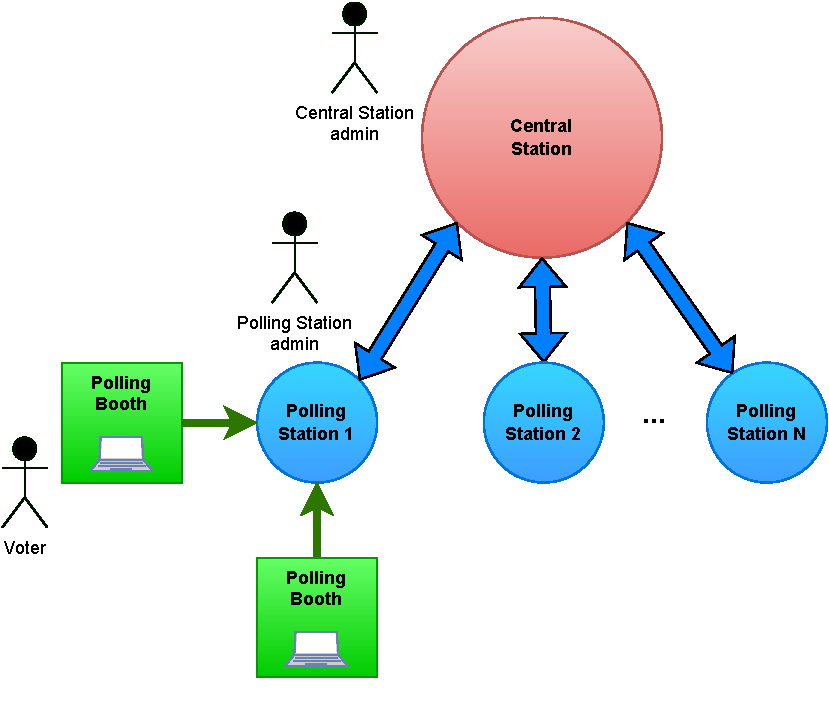
\includegraphics[scale=1]{img/high_lev_arch.pdf}
    \end{center}
    \vspace*{-0.5cm}
    \caption{High level view of the application architecture.}
    \label{fig:high_lev_arch}
\end{figure}




\section{Functional requirements}\label{sec:func_req}
The following functional requirements have been identified:

\subsection*{Voter}
\begin{itemize}
	\setlength\itemsep{1pt}
	\item An anonymous user should be able to login to the platform via private key authentication.
	\item A logged user should be able to express their voting preference via web UI on the electronic device present in the polling station.
\end{itemize}

\subsection*{Polling station admin}
\begin{itemize}
	\item An admin user should be able to login to the admin dashboard via username and password.
	\item An admin user should be able to open the vote.
	\item An admin user should be able to temporarily suspend the vote.
	\item An admin user should be able to close the vote.
	\item An admin user should be able to view statistics related to the vote such as the turnout.
	\item An admin user should be able to manually add people to the list of the voters in particular cases (military, etc.)
\end{itemize}

\subsection*{System}
\begin{itemize}
	\item The system should remember which voters already expressed a vote.
	\item The system should aggregate the votes expressed in the single polling station.
	\item The system should aggregate the total counts of vote for each candidate coming from each of the polling stations.
\end{itemize}

\section{Non-functional requirements}\label{sec:non_func_req}
The application was designed to ensure security aspects which are to be guaranteed during any election, namely:\\
\begin{itemize}
	\item Privacy and vote secrecy
	\item Double voting prevention
	\item Anonymity
	\item Authentication
	\item Authenticity
	\item Unlinkability
\end{itemize}
\hfill \break
\noindent These security aspects are achieved through the use of different means. More in detail:\\
\begin{itemize}
	\item Privacy and vote secrecy have been ensured by means of asymmetric encryption
	\item Double voting prevention is ensured by keeping track in a database of who voted and who did not.
	\item Anonymity and unlinkability are guaranteed by ``splitting" the vote and the voter identity once the former is sent to the central station
	\item Authentication is ensured by face recognition upon entering the polling station and via private key authentication.
	\item Authenticity is achieved via digital signature algorithm
\end{itemize}
%-------------------------------------------------------------------------------
% File: architecture.tex
%
% Author: Marco Pinna
%         Created on 14/07/2022
%-------------------------------------------------------------------------------
\chapter{Architecture}\label{ch:architecture}
This chapter analyses in greater detail the architecture of the application, showing which modules are present where and how they interact with each other. In the second part the structure of the packets exchanged between modules is presented.
\hfill \break


When a voter enters the polling station, the personnel in charge authenticates them via face recognition and personal documents. After checking that the voter is registered to that polling station, they are allowed to enter the polling booth.\\ The voter authenticates themselves again inside the voting booth with an electronic document, such as an electronic identity card. On each polling booth there is a Tomcat instance running, which will serve the web page on which the voter will express their vote.\\
The voters' electronic document will also contain the private key of the voter ($Priv_{vot\_i}$), which will be used to sign the packet containing the vote; the packet signature will be verified on the polling station upon reception with the corresponding voter's public key ($Pub_{vot\_i}$) contained in the \textit{voter} database, to guarantee authenticity and integrity of the vote.\\
\pagebreak
The vote, before being sent over the local network to the polling station server, is encrypted with the public key of the central station ($Pub_{CS}$). The polling station, therefore, is not able to decrypt the vote cast by the voter, and vote secrecy is thus ensured.\\
Once the polling station receives the voter's vote, it sets their corresponding flag \texttt{has\_voted} in the \textit{voter} database to \texttt{true}, to prevent double voting. At this point, the polling station node ``splits" the voter id from the vote and only sends the latter, after signing it with its own private key ($Priv_{PS\_j}$). This ensures the unlinkability of the vote.\\
The central station receives the packet containing the vote, signed by the polling station, and verifies said signature using the corresponding polling station public key ($Pub_{PS\_j}$) which is contained in the \textit{pollingStation} database.\\
Lastly, the vote is saved in the \textit{votes} database in encrypted form. When the voting is over (and only then), the votes will be retrieved from the database and decrypted.

\begin{figure}[H]
    \begin{center}
        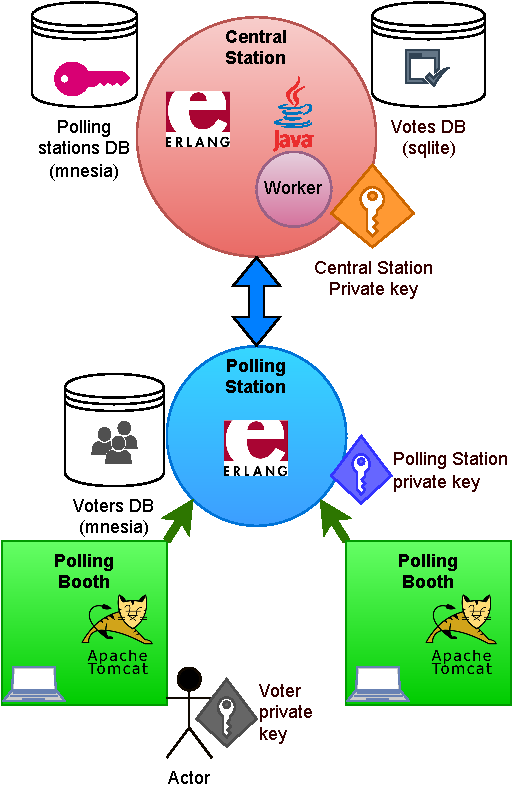
\includegraphics[scale=1]{img/arch_detail.pdf}
    \end{center}
    \vspace*{-0.5cm}
    \caption{A more detailed view of the application architecture.}
    \label{fig:arch_detail}
\end{figure}

\section{Cryptographic scheme}
The whole application was designed to be secure by design from the beginning.\\
In particular, the \textit{elliptic-curve cryptography} (ECC) approach was chosen over RSA because its algorithms are more efficient and yield the same level of security with shorter keys.\\

The two main critical types of packets are the ones containing the vote, which are sent firstly by the polling booth to the polling station and then by the polling station to the central station.\\

\begin{figure}[H]
    \begin{center}
        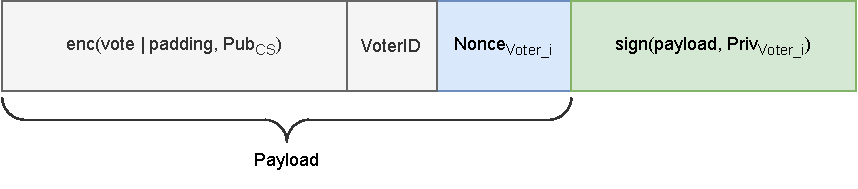
\includegraphics[scale=1]{img/packet1.pdf}
    \end{center}
    \vspace*{-0.5cm}
    \caption{Structure of the \textit{vote} packet sent from the polling booth to the polling station.}
    \label{fig:packet1}
\end{figure}

\begin{figure}[H]
    \begin{center}
        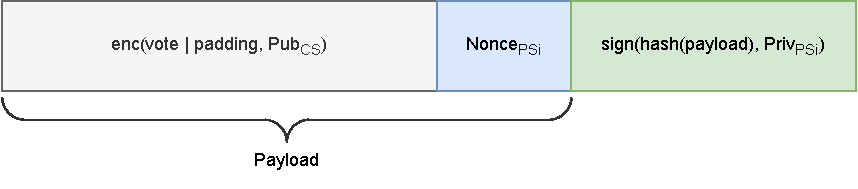
\includegraphics[scale=1]{img/packet2.pdf}
    \end{center}
    \vspace*{-0.5cm}
    \caption{Structure of the \textit{vote} packet sent from the polling station  to the central station.}
    \label{fig:packet2}
\end{figure}

Some additional simplifying hypotheses concerning the security of the operations were made, e.g. further security measures are implemented at network level (firewalls, VPNs, etc.) to prevent packet tampering and sniffing.
%-------------------------------------------------------------------------------
% File: java.tex
%
% Author: Marco Pinna
%         Created on 14/07/2022
%-------------------------------------------------------------------------------
\chapter{Java}\label{ch:java}
The application comprises four Java modules with the following structure:
\hfill \break
\dirtree{%
.1 DVoting.
.2 CentralStation.
.3 src/main/java/it.unipi.dsmt.dvoting.centralstation.
.4 CentralStationDaemon.
.4 CentralStationDashboard.
.4 DatabaseManager.
.4 VotesIterator.
.2 network.
.3 src/main/java/it.unipi.dsmt.dvoting.network.
.4 Network.
.2 WebApp.
.3 src/main/java/it.unipi.dsmt.dvoting.
.4 AccessServlet.java.
.4 AdminServlet.java.
.4 BoothServlet.java.
.4 Candidates.java.
.4 Voter.java.
.4 WebAppNetwork.java.
.2 crypto.
.3 src/main/java/it.unipi.dsmt.dvoting.crypto.
.4 Crypto.
}
\pagebreak
\section*{CentralStation}\label{sec:centralstation}
The \textbf{CentralStation} module runs on the central station and handles the sending and receiving of messages and the interaction with the \texttt{votes} database.\\
\begin{itemize}
	\item The \texttt{CentralStationDaemon} class is always running on the central station for the whole duration of the election. It takes care of receiving from the messages containing the encrypted votes from the polling stations and store them in the database.
	\item The \texttt{CentralStationDashboard} class provides a dashboard meant to be used by the central station admin. It allows them to start/stop the central station daemon and to also get the turnout of the election.
	\item The \texttt{DatabaseManager} class handles the interaction with the \texttt{Votes} database (cfr. \ref{ch:database}).\\
	\item The \texttt{VotesIterator} class extends the \texttt{Iterator} Java util class and it is used when the election is closed and all the votes have to be retrieved from the \texttt{Votes} database.\\
\end{itemize}

\section*{Network}\label{sec:network}
The \textbf{network} module is a utility module which provides to the Java classes the interface to interact with the Erlang modules. It uses the \texttt{com.ericsson.otp.erlang} Java package.

\section*{WebApp}\label{sec:webapp}
The \textbf{WebApp} module runs on each polling station server. 
\begin{itemize}
	\item The \texttt{AccessServlet} class handles the authentication of the voter when they enter the polling station.
	\item The \texttt{AdminServlet} class implements all the administration-related functionalities: it authenticates and logs in the admin and allows them to perform management actions such as suspending, resuming or stopping the vote, search for a specific voter in the database or get the polling station turnout.
	\item The \texttt{BoothServlet} class provides the web page that will be server to the voter when they enter the polling booth.
	\item The \texttt{Candidates} class takes care of asking the official list of candidates to the central station and providing it to the voter in the polling booth.
	\item The \texttt{Voter} class is used to retrieve the voter information stored in the \texttt{voter} Mnesia database (cfr. \ref{ch:database}).
	\item The \texttt{WebAppNetwork} class extends the aforementioned \texttt{Network} class, adding functionalities necessary to the web app.
\end{itemize}

\section*{Crypto}\label{sec:crypto}
The \textbf{crypto} module is a utility module which contains all the cryptography related function use to generate keys, encrypt, decrypt, sign, verify messages, etc.\\
Most of cryptography-related functionalities have been implemented using the \texttt{bouncycastle} Java library, which extends the \texttt{javax.crypto} library by implementing additional schemes and protocols such as PEM and ECIES (\textit{Elliptical Curve Integrated Encryption Scheme}).\\
The curve used by default by the application is the \textit{secp256r1}, but a different one can be chosen (such as \textit{brainpoolP384r1}) by simply changing one line of code in the module.
%-------------------------------------------------------------------------------
% File: erlang.tex
%
% Author: Marco Pinna
%         Created on 14/07/2022
%-------------------------------------------------------------------------------
\chapter{Erlang}\label{ch:erlang}
The application also includes the following Erlang modules:
\hfill \break
\dirtree{%
.1 DVoting.
.2 Erlang.
.3 centralStation.erl.
.3 pollingStation.erl.
.3 monitor.erl.
.3 util.erl.
.3 seggio.erl.
.3 voter.erl.
}

\begin{itemize}

	\item \texttt{centralStation.erl} runs on the central station. It handles the messages received from the polling stations and verifies their signatures. It also replies to requests coming from the polling stations for the list of candidates.
	\item \texttt{pollingStation.erl} runs on each polling station. Its main functionality is to receive the votes from the polling booths, verifying their integrity and authenticity with the voter's public key and updating the \textit{voter} database by setting the corresponding flag.\\
	 It also implements some of the administration functionalities by handling admin commands such as suspend/resume/stop the vote etc.
	 \item \texttt{monitor.erl} acts as a supervisor for the other modules TODO complete
	 \item \texttt{util.erl} contains constants and utility functions.
	 \item \texttt{seggio.erl} contains the functions necessary to interact with the polling station database.
	 \item \texttt{voter.erl} contains the functions necessary to interact with the voters database.

\end{itemize}
%-------------------------------------------------------------------------------
% File: database.tex
%
% Author: Marco Pinna
%         Created on 06/08/2022
%-------------------------------------------------------------------------------
\chapter{Database}\label{ch:database}
A total of three databases have/has been created for the application:
\begin{itemize}
	\item the \texttt{votes} database, which is located in the central node and stores all the votes in encrypted for the whole duration of the election;
	\item the \texttt{polling stations} database, which is also located in the central node and stores the information related to each polling station, included their public keys;
	\item the \texttt{voter} database. Each polling station has its own voter database, containing the information related to each voter who is registered to said polling station. It contains the voters' personal details, necessary for the identification, as well as each voter's public key.
\end{itemize}

\section{Votes database}\label{sec:votes_db}
The \texttt{votes} database is a SQLite database located on the central node. It receives and stores in encrypted form all the votes cast by the voters during the election.\\
The database only consists of one table, \texttt{votes}, whose schema is the following:\\
\begin{figure}[H]
    \begin{center}
        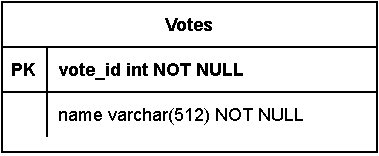
\includegraphics[scale=1]{img/votes_schema.pdf}
    \end{center}
    \vspace*{-0.5cm}
    \caption{Schema of the \texttt{votes} table.}
    \label{fig:votes_schema}
\end{figure}
The interaction with this database is handled by the \texttt{DatabaseManager} Java class which offers an interface to perform CRUD operations.\\
The module that interact with the \texttt{votes} database are the \texttt{CentralStationDaemon} to add the votes to the database and the \texttt{CentralStationDashboard} to obtain the election turnout. %TODO check if something is missing
An example of how the table might appear during the election is the following:

TODO: add example of database

\section{Polling stations database}\label{sec:polling_stations_db}
The \texttt{polling stations} database is a Mnesia database located on the central node. It stores the information related to each polling station.\\
The database only consists of one table, \texttt{pollingStation}, whose schema is the following:\\
\
\begin{figure}[H]
    \begin{center}
        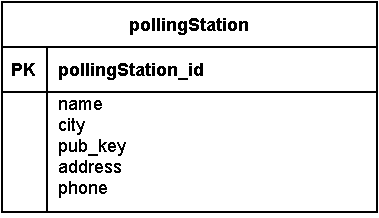
\includegraphics[scale=1]{img/pollingstation_schema.pdf}
    \end{center}
    \vspace*{-0.5cm}
    \caption{Schema of the \texttt{pollingStation} table.}
    \label{fig:pollingstation_schema}
\end{figure}

It is worth noting that ``Mnesia tables \textit{have no built-in type constraints}, as long as you respect the tuple structure of the table iteslf."\footnote{\textit{Learn you some Erlang for great good},Fred Hébert, 2013, p. 514.}.\\
The schema of this table is specified in the Erlang header file \texttt{pollingStation.hrl} while \texttt{pollingStation.erl} offers functions to interact with it, e.g. to add a polling station to the database or to retrieve a polling station public key given its id.\\
An example of how the table might appear during the election is the following:

TODO: add example of database

\section{Voter database}\label{sec:voters_db}
A \texttt{voter} Mnesia database is located on each one of the polling station nodes. Each of them stores the information related to every voter who is registered to that polling station.\\
The database only consists of one table, \texttt{voter}, whose schema is the following:\\
\
\begin{figure}[H]
    \begin{center}
        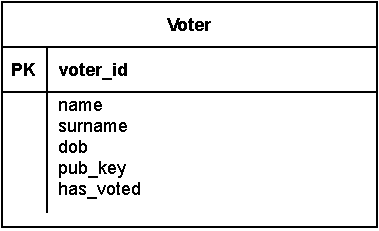
\includegraphics[scale=1]{img/voter_schema.pdf}
    \end{center}
    \vspace*{-0.5cm}
    \caption{Schema of the \texttt{voter} table.}
    \label{fig:voter_schema}
\end{figure}

The schema of this table is specified in the Erlang header file \texttt{voter.hrl} while \texttt{voter.erl} offers functions to interact with it, e.g. to add a voter to the database, to retrieve a voter's public key given their id or to set the flag \texttt{has\_voted} to \textit{true} once the voter has cast their vote.\\
An example of how the table might appear during the election is the following:

TODO: add example of database

%-------------------------------------------------------------------------------
% File: usage.tex
%
% Author: Marco Pinna
%         Created on 14/07/2022
%-------------------------------------------------------------------------------
\chapter{Usage}\label{ch:usage}
TODO

\printbibliography

\end{document}
